\section{Goldstone's theorem}

\begin{figure}[h]
    \centering
    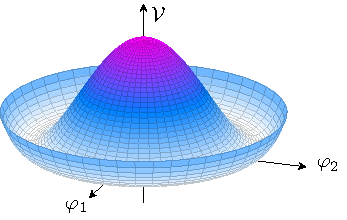
\includegraphics[]{figurer/mexican_hat.pdf}
    \caption{The Mexican hat potential.}
    \label{fig:Mexican hat}
\end{figure}


The ground state of a theory is not necessarily invariant under the symmetry transformations of the theory.
This is exemplified by the linear sigma model,
\begin{equation}
    \Ell[\varphi] 
    = \frac{1}{2} \partial_\mu \varphi_i(x) \partial^\mu \varphi_i(x) - \Ve(\varphi),
    \quad \Ve(\varphi) = - \frac{1}{2} \mu^2 \varphi_i(x)\varphi_i(x)
    + \frac{1}{4} \lambda [\varphi_i(x) \varphi_i(x)]^2.
\end{equation}
The linear sigma model Lagrangian is invariant under the rotation of the $N$ fields,
\begin{equation}
    \varphi_i \longrightarrow \varphi_i' = O_{ij} \varphi_j,
    \quad O^{-1} = O^{T}.
\end{equation}
This is a global, internal and continuous set of transformations, with the infinitesimal form
\begin{equation}
    \varphi_i(x) = \varphi_i(x) + \epsilon \, i t_{ij} \varphi_j(x)
\end{equation}
The group of all such transformations form the Lie group $O(N)$. (SKRIVE APPENDIX OM LIE GRUPPER?)
If we assume the ground state $\varphi_{0}$ is translationally invariant, then it is given by minimizing the effective potential.
The first approximation of this is given by the classical potential, $\Ve$.
For $N=2$, this is the famous ``Mexican hat''-potential, as illustrated by \autoref{fig:Mexican hat}.
The ground state is therefore given by any of the values along the brim of the potential.
If we, without loss of generality, choose $\varphi = (0, v)$ as the ground state, then any symmetry transformation will change this state.
We say that the symmetry has been \emph{spontaneously broken}.
We can express this mathematically as
\begin{equation}
    t_{ij} \ex{ \varphi_i}_0 \neq 0.
\end{equation}

If we take the constraint \cref{effective equation of motion}, differentiate with respect to $\varphi_j(y)$ and evaluate in the vacuum, we get
\begin{equation}
    \int \dd^4 x \, \fdiff{\Gamma[\varphi_0]}{\varphi_j(y), \varphi_i(x)}
    t_{ik} \ex{\varphi_k}_0 = 0.
\end{equation}
In \autoref{Effective action inverse propagator}, we found that the second derivative of the effective action is the inverse propagator.
The momentum space propagator is therefore
\begin{equation}
    i \delta(0) \tilde D_{ji}^{-1}(p) 
    = \int \dd^4 x \, e^{-i p x}  
    \fdiff{\Gamma[\varphi_0]}{\varphi_j(0), \varphi_i(x)}.
\end{equation}
(CHECK THAT)
If we assume the ground state is independent of space-time, we get
\begin{equation}
    \tilde D^{-1}_{i j}(p=0) \, t_{j k} \ex{\varphi_k}_0 
    = \diffp{\Veff}{\varphi_i, \varphi_j} \, t_{j k} \ex{\varphi_k}_0  
    = 0.
\end{equation}
If the symmetry transformation $\varphi_i \rightarrow \varphi_i + i \epsilon t_{ij} \varphi_j$ remains unbroken, then this is trivial, as $t_{ij} \ex{\varphi_j }_0= 0$.
However, if it is a broken symmetry, then by definition $t_{ij} \ex{\varphi_j }_0 \neq 0$.
In that case, $t_{ij} \ex{\varphi_j}_0$ has a zero eigenvalue of the inverse propagator, at $p = 0$.
In other words, the system contains a zero-mass particle, a Goldstone boson.\footnote{ The particles are bosons due to the bosonic nature of the transformations, $t$. If the generators are Grassmann numbers, the resulting particle, called a goldstinos, are fermions.}

The set of continuous symmetry transformations, 
\begin{equation}
    G = \setbuilder{g}{g(\varphi) = \varphi', \, S[\varphi'] = S[\varphi], \D \varphi' = \D \varphi },
\end{equation}
form a Lie group.
An $N$ dimensional Lie group can be parametrized by $N$ real numbers.
The set of generators, $\mathfrak{g} = \setbuilder{t}{g(\varphi) = \varphi + \epsilon i t(\varphi) + \Oh{\epsilon}}$, is called a Lie algebra, and forms a vector space.\footnote{The factor $i$ is a physics convention, and differs from how mathematicians define generators of a lie group.}
$\mathfrak{g}$ is an $n$ dimensional Lie group, and thus has a basis of $n$ vectors, $t^\alpha$.
The finite transformations of $G$ are generated by elements in $\mathfrak{g}$ through the exponential map, $g = \exp{i \theta^\alpha t^\alpha }$.
A generator $t^\alpha$ corresponding to a broken symmetry is called a \emph{broken generator}.
Each broken generator corresponds to a zero-eigenvalue eigenvector.
In Lorentz invariant systems this corresponds to one massless mode per broken generator.
The remaining, unbroken generators forms a subgroup $H \subset G$, so the number of zero-mass modes are $n_G = \dim(G) - \dim(H)$.

\begin{figure}[h]
    \centering
    \begin{subfigure}{0.54\textwidth}
        \centering
        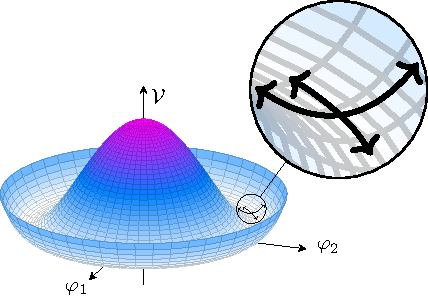
\includegraphics[]{figurer/mexican_hat_zoom.pdf}
        \caption{Excitations along the brim does not cost any energy.}
        \label{fig:Mexican hat zoom}
    \end{subfigure}
    \begin{subfigure}{0.45\textwidth}
        \centering
        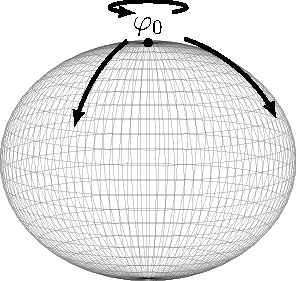
\includegraphics[]{figurer/sigma_ground_state.pdf}
        \caption{Excitations for the $N=3$ sigma model. Two of the symmetries are broken, while rotations around the groundstate leaves the system unchanged.}
        \label{fig:ground state manifold}
    \end{subfigure}
\end{figure}

The Mexican hat potential gives an intuition for the Goldstone mode.
In the case of the two-dimensional sigma model, the symmetry of the Lagrangian are rotations in the plane.
As the ground stat is along the ``brim'' of the hat, this rotational symmetry is broken.
Any excitations in this direction, however, does not cost any energy, which is indicative of a massless mode.
This is illustrated in \autoref{fig:Mexican hat zoom}.
In this example, the original symmetry group is one dimensional, so there is no unbroken symmetries.
If we instead consider the three-dimensional linear sigma model, which has a three-dimensional symmetry group, rotations of the sphere.
The ground state manifold, the set of all the degenerate ground states, is then a sphere.
When the system chooses one single ground state, this symmetry is broken, but only for two of the generators. 
The generator for rotations around the ground state leaves the that point unchanged, and is thus an unbroken symmetry.
This is illustrated in \autoref{fig:ground state manifold}.

